\documentclass[utf8]{beamerDMS}
%% OTHER USEFUL SETTINGS
%% no ToC for conference presentation
%\documentclass[utf8, hideSidebar]{beamerDMS}
%% printing slides
% \documentclass[utf8, xcolor=table, trans, slideTotalNumber, emptyFootings, hideResults]{beamerDMS}
%% presentation - basically defaults
% \documentclass[utf8, xcolor=table, beamer, showResults]{beamerDMS}
%% start in fullScreen
% \hypersetup{pdfpagemode=FullScreen}
%% DMS logo instead of MUL on individual slides
% \setFrameLogo{graphics/institute-logo}

\title[Short title]{Very long title of the whole presentation which could span over more lines}
\author[First A. {\sl et al.}]{First Author\aff{1,2}, Second Author\aff{2} and Last Author\aff{3}} 
\institute{
  \aff{1}First address\\
  \aff{2}Second address\\
  \aff{3}Third address}
\email{first.author@unileoben.ac.at}
\lecture{Name of the course}
\conference{Name of the conference}
\date{Date}
\additionsToTitlePage{
  \put(0,1.2){\parbox[t]{12cm}{%
      \centering%
      \usebeamerfont{institute}{\color{DMSaddress} conference name
    }}%
}}

\begin{document}

\begin{frame}
\titlepage
\end{frame}

\section{Introduction}
\subsection{First Slide}
\literature{
  L. Huber, B. Grabowski, M. Militzer, J. Neugebauer, and J. Rottler, {\em Comput. Mater. Sci.} {\bf 118}, 259 (2016)\\
  D. Holec, N. Abdoshahi, S. Mayer, and H. Clemens, {\em Materials} {\bf 12}, (2019)}
\begin{frame}{Hokus pokus}
\begin{block}{A Block}
  This is \alert{a block}:
  $$a^2+b^2=\Alert{c^2}\, \quad \sin\alpha=\frac{b}{c}$$
\end{block}

\begin{minipage}{5cm}
  \begin{itemize}
    \item first one
    \example second one
    \item last one
  \end{itemize}
\end{minipage}
\begin{minipage}{5cm}
  \begin{block}{}
    
\includegraphics[height=1cm]{graphics/logo_MUL_M}
  \end{block}
\end{minipage}

normal text afterwards\dots
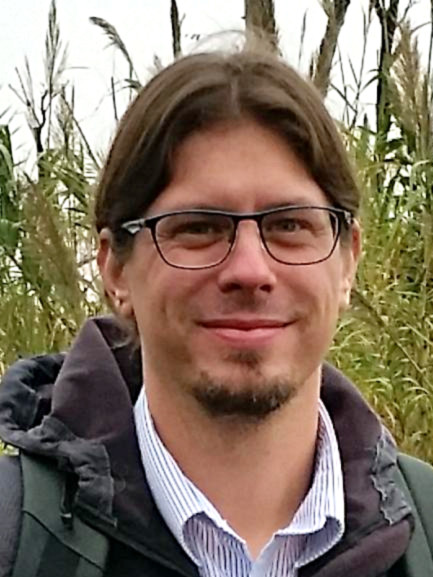
\includegraphics[height=2cm]{figs/david}
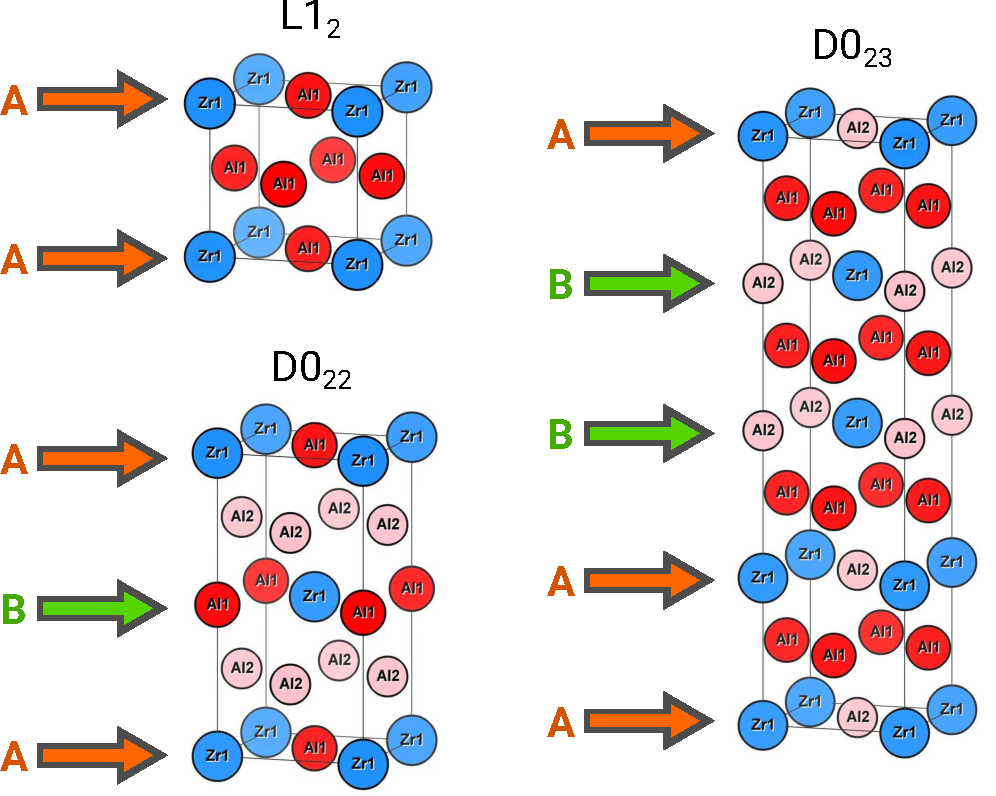
\includegraphics[height=2cm]{figs/structures}

\unitlength=1cm
\begin{picture}(0,0)
  \put(0,0){
\includegraphics[width=3mm]{graphics/logo_MUL_M}}
  \put(11,0){
\includegraphics[width=5mm]{graphics/logo_MUL_M}}
  \put(11,3){
\includegraphics[width=5mm]{graphics/logo_MUL_M}}
\end{picture}
\end{frame}

\subsection{How to use \texttt{framegrid}}
\begin{frame}{Abra abra kadabra}
	\onslide<1->
		content...
		And eve ever more content
		\begin{figure}
			\centering
			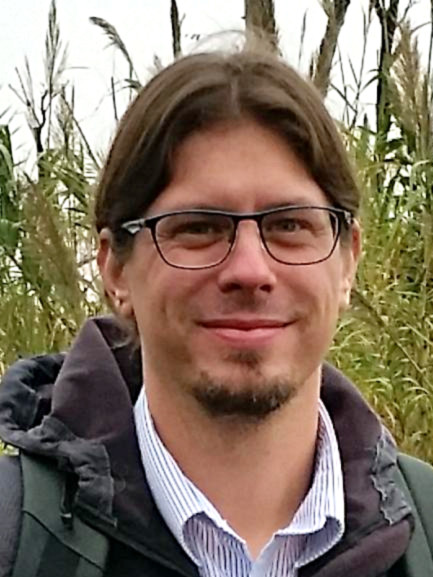
\includegraphics[height=4cm]{figs/david}
			\caption{This is David. Lets' make him new his glasses with \texttt{framegrid}}
		\end{figure}
	\onslide<2>
		\begin{overdraw}
			\framegrid
		\end{overdraw}
	\onslide<3>
	\begin{overdraw}
		\framegrid
		\draw [red, very thick] (8.8, 5.7) circle (0.25);
		\draw [red, very thick] (9.55, 5.7) circle (0.25);
		\draw [red, very thick] (9.05, 5.7) -- (9.3, 5.7);
	\end{overdraw}
	\onslide<4>
	\begin{overdraw}
		\draw [red, very thick] (8.8, 5.7) circle (0.25);
		\draw [red, very thick] (9.55, 5.7) circle (0.25);
		\draw [red, very thick] (9.05, 5.7) -- (9.3, 5.7);
	\end{overdraw}

\end{frame}

\end{document}
